% Vorgaben Assignment aus Studienheft SQL03
% Formatvorgaben fuer den Text
% Umfang: 8 - 10 Seiten (inkl. Abbildungen und Tabellen, aber ohne Deckblatt, % Gliederung und Literaturverzeichnis, Eidesstattliche Erklaerung)
% Zeilenabstand: 1,5
% Schriftart: frei
% Schriftgrad: 12 pt
% Variablen, physikalische Groessen und Funktionszeichen werden kursiv gedruckt.
% Korrekturrand: links: 4,5 cm, rechts 2,0 cm, oben und unten jeweils 3,0 cm
% Deckblatt: (Adresse, AKAD-E-Mail-Adresse, Immatrikulationsnummer, Modul-
% bezeichnung, Thema, Datum, Felder für Korrektor)
% Gliederung (1 Seite)
% Literaturverzeichnis (3 - 5 Literaturquellen  z. B. Lehrbuecher, aktuelle Fachartikel recherchieren)
% Eidesstattliche Erklaerung (unterschrieben und fest eingebunden)
% Bearbeitungsdauer: 2 Monate


\documentclass[a4paper,12pt]{article}
\usepackage[ngerman]{babel}
\usepackage[nottoc]{tocbibind} % Anzeigen des Literaturverzeichnisses im TOC
\usepackage{epsfig}
\usepackage{times}
\usepackage{supertabular}
\usepackage{wrapfig}
\usepackage{multirow}
\usepackage[onehalfspacing]{setspace}
\usepackage{listings}
\usepackage{mathptmx}
\usepackage{geometry}
\usepackage{floatflt}
\usepackage{helvet}
\usepackage{courier}
\usepackage{setspace}
\usepackage{textcomp}
\usepackage[T1]{fontenc}
\usepackage[utf8]{inputenc}
\usepackage{fancyhdr}
\usepackage{float} % Notwendig fuer figure[h]
\usepackage[printonlyused]{acronym}
\usepackage{makeidx}
\usepackage[activate={true,nocompatibility},final,tracking=false,kerning=true,spacing=true,factor=1100,stretch=20,shrink=20]{microtype}

\makeindex

\newif\iflistoffigures
\newif\iflistoftables
\newif\ifacronym

%Titel
\newcommand*{\Titel}{Daten sind das Öl des 21. Jahrhunderts} 

%Betreff
\newcommand*{\Betreff}{Assignment} 

%Betreuer
\newcommand*{\Betreuer}{Prof. J. Anton Illig} 

%Vor- und Nachname
\newcommand*{\Name}{Stefan Waidele}

%Straße und Hausnummer
\newcommand*{\Strasse}{Ensisheimer Straße 2} 

%Plz und Ort
\newcommand*{\PlzOrt}{79395 Neuenburg am Rhein} 

%Immatrikulationsnummer
\newcommand*{\Immatrikulationsnummer}{102 81 71}

%Email 
\newcommand*{\Email}{Stefan@Waidele.info} 


% Verzeichnisse (Wenn nicht benötigt, Zeile mit % auskommentieren oder löschen

%% Abbildungsverzeichnis 
\listoffigurestrue
%% Tabellenverzeichnis
%\listoftablestrue
%% Abkürzungsverzeichnis
\acronymtrue

% Wittwen und Waisen verhindern
\clubpenalty10000
\widowpenalty10000
\displaywidowpenalty=10000

\usepackage[flushmargin,hang,ragged]{footmisc}
\usepackage{lmodern} %Type1-Schriftart für nicht-englische Texte
\usepackage{fancyhdr}

\usepackage[
	pdftitle={\Titel},
	pdfsubject={WIN03 -- Innovative Themen der Wirtschaftsinformatik},
	pdfauthor={Stefan Waidele},
	pdfkeywords={akad, win03, assignment, wirtschaftsinformatik}
	hyperfootnotes=false,
	colorlinks=true,
	linkcolor=black,
	urlcolor=black,
	citecolor=black
]{hyperref}

%\renewcommand{\familydefault}{\rmdefault}
\renewcommand{\bflabel}[1]{\normalfont{\normalsize{#1}}\hfill}

%% Definition for Codeschnipsel im Fließtext
\newcommand{\code}{\texttt}
% \newcommand{\buzz}{\textit}
\newcommand{\buzz}{\textit}

\newcommand{\todo}[1]{\fbox{\parbox{\textwidth}{\textbf{To do:} #1}}}
%\newcommand{\myref}[1]{„\ref{#1}~\nameref{#1}“}
\newcommand{\myref}[1]{\textit{\ref{#1}~\nameref{#1}}}

%% Für Codeblöcke mit Syntax-Highlighting
%% http://www.ctan.org/tex-archive/macros/latex/contrib/minted/
\usepackage{minted}
\definecolor{bg}{rgb}{0.95,0.95,0.95}


\makeatother

\geometry{a4paper, left=45mm, right=20mm, top=30mm, bottom=30mm}
\pagenumbering{roman}

\begin{document}
	
\parskip=1em
\parindent=0cm

%description: Deckblatt in Deutsch
%% Basierend auf einer TeXnicCenter-Vorlage von Tino Weinkauf.
%% sowie der akad-vorlage von Daniel Falkner
%%%%%%%%%%%%%%%%%%%%%%%%%%%%%%%%%%%%%%%%%%%%%%%%%%%%%%%%%%%%%%

%%%%%%%%%%%%%%%%%%%%%%%%%%%%%%%%%%%%%%%%%%%%%%%%%%%%%%%%%%%%%
%% Deckblatt
%%%%%%%%%%%%%%%%%%%%%%%%%%%%%%%%%%%%%%%%%%%%%%%%%%%%%%%%%%%%%
%%
%% ACHTUNG: Sie benötigen ein Hauptdokument, um diese Datei
%%          benutzen zu können. Verwenden Sie im Hauptdokument
%%          den Befehl "\input{dateiname}", um diese
%%          Datei einzubinden.
%%

\begin{titlepage}

%\thispagestyle{empty}

\vspace{5cm}

\Name \\ 
\Strasse \\ 
\PlzOrt\\ 
\href{mailto:\Email}{\Email}

AKAD University\\
Immatrikulationsnummer: \Immatrikulationsnummer

\vfill

\begin{tabbing}
Modul WIN03 --- \=Innovative Themen der Wirtschaftsinformatik\\ 
				\>Assignment
\end{tabbing}

\LARGE
\textsc{Web 3.0 \\Daten sind das Öl des 21. Jahrhunderts}\\

\vfill

\normalsize

Betreuer: \Betreuer

Entwurf vom \today %%Datum der Abgabe - am besten selbst reinschreiben.

\vfill


\includegraphics[width=3cm]{akad_logo.png}

AKAD University

\end{titlepage}

\normalsize


\normalsize

\begin{spacing}{1.0} % Verzeichnisse werden mit einzeiligem Abstand gesetzt
\parskip=0em
\newpage

% Inhaltsverzeichnis
\setcounter{tocdepth}{2}
\tableofcontents 
\newpage

% Abbildungsverzeichnis
\iflistoffigures
\listoffigures 
\newpage
\fi

% Tabellenverzeichnis
\iflistoftables
\listoftables 
\newpage
\fi

% Abkürzungsverzeichnis
\ifacronym
\section*{Abkürzungsverzeichnis}
\addcontentsline{toc}{section}{Abkürzungsverzeichnis} 
\begin{acronym}[\hspace{5cm}]
	\acro{CAPTCHA}{Completely Automated Public Tourint Test to Tell Computers and Humans Apart}
	\acro{CSS}{Cascading Style Sheets}
	\acro{DDoS}{Distributed Denial of Service}
	\acro{DoS}{Denial of Service}
	\acro{ERP}{Enterprise Resource Planning}
	\acro{HTML}{Hypertext Markup Language}
	\acro{HTTPS}{Hypertext Tranfsfer Protocol Secure}
	\acro{HTTP}{Hypertext Tranfsfer Protocol}
	\acro{IoT}{Internet of Things}
	\acro{OWASP}{Open Web Application Security Project}
	\acro{PDO}{PHP Data Objects}
	\acro{SCM}{Supply Chain Management}
	\acro{SQL}{Structured Query Language}
	\acro{WWW}{World Wide Web}
	\acro{XSS}{Cross Site Scripting}

%%
%	
%	\acro{}{}
%	\acro{}{}
%	\acro{}{}
%	\acro{}{}
%	\acro{}{}
%	\acro{}{}
%	\acro{}{}
%	\acro{}{}
	\acro{Test}{Wird nicht im Text verwendet und taucht auch nicht im Verzeichnis auf}
\end{acronym}

\fi

\parskip=1em
\end{spacing} 

\clearpage

\newcounter{romanPagenumber} 
\setcounter{romanPagenumber}{\value{page}} % Roemische Seitenanzahl speichern.


\pagestyle{fancy}
\fancyhead{}
\fancyhead[LO,RE]{\textsc{\Titel}}
\fancyhead[RO,LE]{\thepage}
\fancyfoot[CO,CE]{}
\setlength{\headheight}{15pt}

% \nocite{*} 

\pagenumbering{arabic}

\begin{spacing}{1.5} % Zeilenabstand: 1,5 fuer den Textteil

\section{Einleitung}
\label{sec:einleitung}

\subsection{Begründung der Problemstellung}

Technologien rund um das Schlagwort \buzz{Big Data} sind laut Gartner die großen Triebfedern in der Informationstechnologie\footnote{vgl. \cite{gartner2014}}. Durch Entwicklungen wie \buzz{Internet of Things} und \buzz{Ubiquitous Computing} werden die in naher Zukunft die generierte Datenmenge als auch die Anzahl der verarbeitenden Instanzen in den nächsten Jahren wohl deutlich zunehmen.

Die steigende Menge der Daten macht eine systematische Aufbereitung der anfallenden Daten hin zu repräsentiertem Wissen möglich und notwendig. Das semantische Web, oder auch \buzz{Web 3.0}, verspricht Struktur in die Datenmenge zu bringen. Die Erwartungen, aber auch die Befürchtungen gegenüber den entsprechenden technischen Fortschritten sind immens.

\subsection{Ziele dieser Arbeit}

\textbf{Ziel dieser Arbeit ist es, die momentanen Entwicklungen der Datenbeständen hin zum semantischen Web und deren Auswirkungen auf Wirtschaft und Gesellschaft mit den durch die Industrielle Nutzung des Öls im 20. Jahrhundert zu vergleichen.}

Hierzu werden zunächst im Kapitel~\myref{sec:grundlagen} die für diese Arbeit relevanten Begriffe und Konzepte definiert, bevor im Kapitel~\myref{sec:hauptteil} die Auswirkungen der Technologien auf Wirtschaft und Gesellschaft beschrieben werden.

\todo{An die tatsächliche Arbeit anpassen}

\subsection{Abgrenzung}

Der Augenmerk dieser Arbeit liegt auf den behandelten Konzepten und Technologien der Informationstechnologie. Die Entsprechungen in der Ölindustrie werden nicht in der gleichen Tiefe erörtert und belegt werden, sondern beschränken sich auf generelle Aussagen und Ansichten.

\todo{An die tatsächliche Arbeit anpassen}

\section{Grundlagen}
\label{sec:grundlagen}

\subsection{Betrachtung von Erdöl}

Bei Erdöl handelt es sich um den wichtigsten Energieträger des 20. Jahrhunderts bis hin zur Gegenwart. Durch Erdöl wurden viele technologische Entwicklungen begünstigt oder gar erst möglich gemacht. Durch systematische Aufbereitung in Reffinerien sind neben den offensichtlichen Anwendungen wie der Nutzung als Schmier-- und Kraftstoff für Mobilität und Maschinen oder zur Wärmegewinnung sind viele weitere Anwendungen möglich, ohne die die moderne Gesellschaft nur schwer vorstellbar wäre\footnote{z.b. Kunststoffe und Lacke, welche zum großen Teil auf Erdöl basieren, oder auch die Reichweite, die Fahrzeuge wegen der hohen Energiedichte von Benzin bzw. Diesel erzielen.}.

Die Wertschöpfungskette rund um Erdöl gliedert sich in die Phasen des Finden bzw. Förderns, des Sammelns bzw. Aufbereitens und in die anschließende Nutzung in diversen Endprodukten, vom Treibstoff bis hin zu diversen Kunsstoffen.
Dabei gilt, dass Erdöl zwar in großen Mengen\footnote{Ob diese Mengen, speziell im Vergleich zum weltweiten Verbrauch, tatsächlich immer noch groß sind, wird z.T. bezweifelt}, aber nicht unbegrenzt zur Verfügung steht. 

Die Auswirkungen des Erdöls auf Technologie, Wirtschaft, Gesellschaft und Politik des 20. Jahrhunderts sind enorm. Erdöl ermöglichte großen Reichtum von Unternehmen und Staaten, aber verursachte auch Krisen und Kriege.

\subsection{Definition: Daten, Information, Wissen}
\label{defwissen}

In dieser Arbeit sollen die folgenden Definitionen gelten: Ein \buzz{Datum} ist eine formalisierte Sachverhaltsaussage, ohne inhärente Bedeutung (z.B. „23°C“). Durch Interpretation im Kontext kann daraus eine \buzz{Information} werden (z.B. „Die Außentemperatur beträgt 23°C“)\footnote{vgl. \cite{kfk}, Seite 40}. Durch Vernetzung mehrerer Informationen miteinander, aber auch durch Erfahrung kann \buzz{informatives Wissen} entstehen (z.B. „Das Wetter ist schön“)\footnote{vgl. \cite{pnik}, Seite 106}. 

In weiteren Verfeinerungsschritt entsteht dann \buzz{handlungsorientiertes Wissen}, (z.B. „Ich benötige beim Nachmittagsspaziergang keinen Pullover“) das dann zu einer konkreten Entscheidung führen kann (z.B. „Ich lasse den Pullover zu Hause.“)\footnote{vgl. \cite{taylor}, Seite 342}.

\subsection{Definition: Web 1.0, Web 2.0}

Unter \buzz{Web 1.0} versteht man das \ac{WWW} wie es ursprünglich entwickelt wurde: Eine Menge von statischen Daten, die miteinander auf willkürliche Weise verknüpft werden konnten. Die Auszeichnungssprache \ac{HTML} ermöglicht es Autoren, bestimmte Abschnitte zu kennzeichnen. Schon hier gibt es unterschiedliche Informationsgehalte der Auszeichnungen: Während \code{<b>…</b>} lediglich aussagt, dass der ausgezeichnete Abschnitt in fetter Schriftart angezeigt werden soll, ist eine mit \code{<h1>…</h1>} ausgezeichnete Überschrift tatsächlich als solche zu erkennen. Auch wenn die dadurch gewonnene Information für ein automatisch erstelltes Inhaltsverzeichnis schon nützlich sein kann, wird hier keine Aussage bzgl. des eigentlichen Inhalts getroffen. Somit sind die Dokumente des Web 1.0 dem Bereich der \buzz{Daten} zuzuordnen. Die darin enthaltenen Informationen bzw. das darin enthaltene Wissen ist erst zugänglich, wenn die Daten durch Menschen gelesen und ausgewertet werden\footnote{vgl. \cite{alkhatib}, Seite xvi}.

Durch die Technologien des \buzz{Web 2.0} werden die Daten i.d.R. in Datenbanken vorgehalten und die Webseiten erst bei Abruf generiert. Durch die Popularität von Werkzeugen wie Blogs und Wikis sind deutlich mehr Menschen an der Erstellung der Inhalte beteiligt. Weitere Daten werden durch Techniken rund um das \buzz{\ac{IoT}} und \buzz{Ubiquitous Computing} automatisch erfasst. Diese Daten mit sogenannten \buzz{Meta--Daten} angereichert. Hierdurch wird in maschinenlesbarer Form angegeben, welche Informationen die Dokumente enthalten. Neben vom Autor selbst zugeordneten \buzz{Tags} und \buzz{Kategorien} kommen auch automatisch generierte Meta--Daten hinzu. Beispiele hierfür sind etwa das Veröffentlichungsdatum, Beziehungen zu anderen Dokumenten\footnote{Realisiert durch sog. Backtracks -- Wer verlinkt auf dieses Dokument?} oder Geoinformationen (Wo wurde das Dokument erstellt). Inzwischen werden auch die Stimmung des Autors erfragt (z.B. bei Runtastic–Aktivitäten) oder ermittelt (z.B. bei Facebook--Einträgen). Die durch Daten und Meta--Daten erzielte Informationsstufe ist deutlich über der von \buzz{Web 1.0}, unterliegt aber deutlichen Schwankungen je nach Dienst bzw. Nutzereingaben.

\subsection{Web 3.0 = Web 2.0 + Semantik = Semantisches Web}

„\buzz{Semantik}, auch \buzz{Bedeutungslehre}, nennt man die Theorie oder Wissenschaft von der Bedeutung der Zeichen. Zeichen können in diesem Fall Wörter, Phrasen oder Symbole sein. Die Semantik beschäftigt sich typischerweise mit den Beziehungen zwischen den Zeichen und den Bedeutungen dieser Zeichen.“\footnote{cite{wp:semantik}}

Im \buzz{Web 3.0} werden die Daten bzw. Informationen des Web 2.0 durch Beifügung von Bedeutung zu Information bzw. informativem Wissen veredelt\footnote{vgl. \cite{nyt:markoff}}. Hierdurch soll es möglich werden, die schnell steigenden Datenmengen sinnvoll zu nutzen\footnote{vgl. \cite{tsp:tolksdorf}}. Die Bezeichnung \buzz{semantisches Web} ermöglicht eine Abgrenzung gegenüber anderen Interpretationen des Buzzwords \buzz{Web 3.0}, wie sie z.T. im Marketing\footnote{z.B. „Web 3.0 marketing is the convergence of new technologies and rapidly changing consumer buying trends.“ in \cite{web3market}, Abschnitt „What is Web 3.0 Marketing?“} oder in der Politikwissenschaft\footnote{z.B. „Is this Web 3.0? Not a tech-upgrade, a smarter algorithm, slicker fibre optic or better Bluetooth beam. Instead, Web 3.0 as in an outcome, the demonstrated consequences of being able to access information?“ in \cite{web3pol}, Abschnitt „Web 3.0: Regime Change“} zu finden sind.

\section{Die Bedeutung der Daten}

\subsection{Metadaten}

zum Zeitpunkt der Erzeugung der Daten
oder on the fly (Genutzter Plattenplatz, etc.)

entweder in der Datei (EXIF) oder extern .info bei Amiga

Auch Textverarbeitungsdokumente, etc.,

\subsection{Semantisches Markup}

Beschreibung der Daten außerhalb der Datei

\subsection{Automatische Informationsgewinnung}

z.B. Gesichtserkennung

\subsection{Automatische Wissensgewinnung}

Durch Verknüpfung von Informationen kann Wissen generiert werden:\\
Person A ist auf einem Bild zusammen mit Person B zu sehen (Gesichtserkennung). Die Geoinformation und Uhrzeit (EXIF--Tags) zeigen, dass das Foto auf einer Veranstaltung aufgenommen wurde, das zu diesem Zeitpunkt an diesem Ort statt fand (Semantisches Markup der Veranstaltung).

Daraus kann auf politische Gesinnung oder Trinkfreudigkeit von Person A geschlossen werden.
\section{Web 3.0 --- Das Semantische Web}
\label{sec:hauptteil}

\subsection{Daten als Handelsware}
\label{handelsware}

Sowohl Daten als auch Information und Wissen werden ähnlich wie physische Güter gehandelt. Hierbei bestehen aufgrund der Intangibilität und der Irreveribilität von Transaktionen deutliche Unterschiede zum Handel mit Erdöl.\footnote{vgl. \cite{wiener}, Seite 117} Da jedoch ein realer Markt für virtuelle Güter besteht und diese dort einen Preis erzielen, stellen Daten und die daraus gewonnenen Produkte auch Handelswaren dar.\footnote{vgl. \cite{wiener}, S115}

Der Wert dieser Ware lässt sich jedoch nicht beliebig erhalten, da dieser durch Weiterverbreitung bzw. Veränderungen in durch die Daten beschriebenen Realität abnehmen kann.\footnote{vgl. \cite{wiener}, Seite 113 bzw. 122}

\subsection{Einschätzungen von Analysten und der Politik}
\label{politik}

Gartner rechnet mit einem Anstieg der mit dem Internet verbundenen Geräte um das Fünffache  von fast fünf auf über 25 Milliarden Geräten im Jahr 2020.\footnote{vgl. \cite{gartneriot}, Tabelle 1} Zusätzlich zu den durch Herstellung und Vertrieb dieser Geräte erzielten Wertschöpfung wird in 2020 die Inanspruchnahme von Dienstleistungen im Wert von 263 Milliarden Dollar erwartet.\footnote{vgl. \cite{gartneriot}, Absatz 3}

Von Politikern auf verschiedenen Ebenen wird der Themenbereich \buzz{Big Data} als sehr wichtige Wachstumsfeld eingeschätzt. So erklärt z.B. die EU--Kommissarin für die Digitale Agenda Needie Kroes: „Daten sind Antrieb und Grundlage für die Wirtschaft der Zukunft. Organisationen jeder Art [...] benötigen Daten als Bausteine, um leistungsfähiger zu werden.“\footnote{Zitiert nach \cite{bd25}} und rechnet mit 100.000 neuen Arbeitsplätzen in der Datenverarbeitungsbranche. Durch ein Förderprogramm in Höhe von 2,5 Milliarden Euro soll die soll die Entwicklung von Techniken und Diensten zur Verarbeitung großer Datenmengen durch Einsatz von künstlicher Intelligenz gefördert werden.\footnote{vgl. \cite{bd25}}

Das Umwelt--Bundesamt kümmert sich um Nachhaltigkeit nicht nur bei der Hardware, sondern auch bei Software und den erhobenen Daten. „Wachsende Datenmengen und überdimensionierte Programme erfordern den beständigen Ausbau von IT-Netzen, Datenspeichern und Rechenkapazitäten. Höchste Zeit also, die Diskussion über Nachhaltige Software anzustoßen.“\footnote{\cite{fns}} 

Somit werden in der Politik die gleichen Ziele verfolgt wie im Bezug auf die Ölbranche: Sicherung bzw. Steigerung des Marktanteils, Erzielung von möglichst positiven Effekten auf den Arbeitsmarkt sowie die bestmögliche Vermeidung der negativen Auswirkungen auf Umwelt und Gesellschaft.

\subsection{Auswirkungen auf die Gesellschaft}

Schon heute drehen sich die meisten der regelmäßig ausgeführtem Aktivitäten im Internet um \buzz{Informationen}\index{Information} oder gar \buzz{Wissen}\index{Wissen}, nicht um \buzz{Daten}\index{Daten}. So sind 56\% der im Digitalindex 2014 befragten Deutschen überzeugt, im Internet die automatisch die aktuellsten Informationen zu finden, 60\% sucht benötigte Informationen zuerst im Netz\footnote{vgl. \cite{d21}, Seite 6}. Die Erwartungen bzgl. Aktualität und Informationsgehalt an das \buzz{World Wide Web}\index{Web!World Wide} sind also sehr hoch. 

Unter den Top 10 der regelmäßig durchgeführten Tätigkeiten der Befragten im Web finden sich die informationsorientierten Tätigkeiten „nach Inhalten/Informationen suchen“ auf Platz eins, „über aktuelle Ereignisse des Wohnorts informieren“ auf Platz 6 und die Erfassung eigener Daten auf dem 10. Platz.\footnote{vgl. \cite{d21}, Seite 37} Weitere Tätigkeiten wie „Soziale Netzwerke nutzen“ (Platz 7) bzw. „Online--Videos ansehen“ (Platz 3) sowie „Online--Shopping“ (Platz 2) nutzen Internetangebote, die per Design sehr gut mit Taxonomien, Meta--Daten und Verknüpfungen ausgestattet sind.

\begin{figure}[H]
\begin{center}
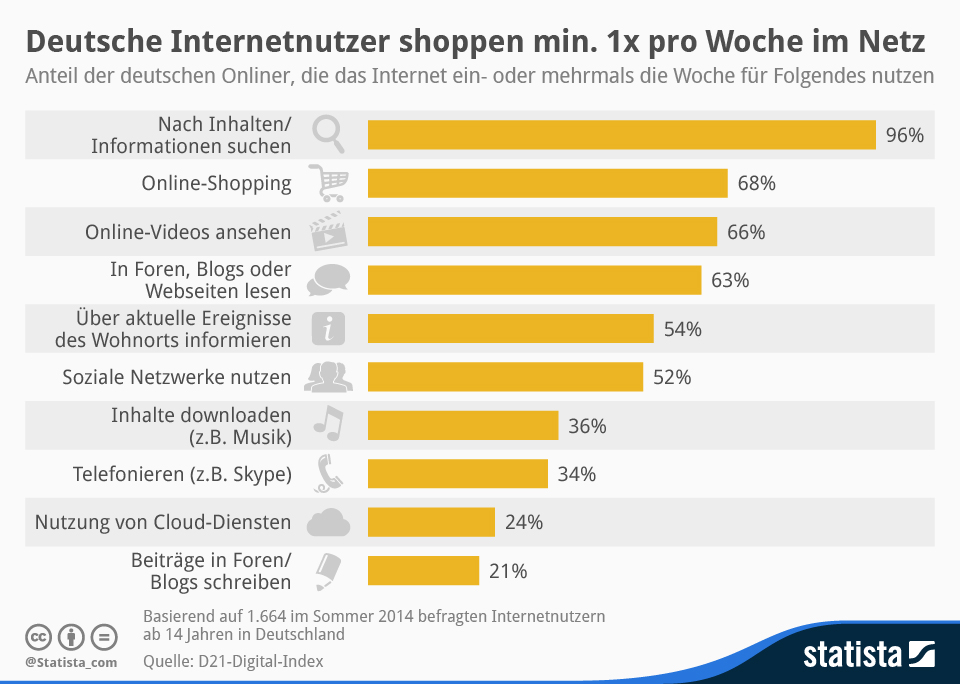
\includegraphics[width=0.67\textwidth]{inetnutzung.jpg}
\caption[Internetnutzung in Deutschland 2014]{Internetnutzung in Deutschland 2014\protect\footnotemark}
\label{pic:inetnutzung}
\end{center}
\end{figure}
\footnotetext{\cite{d21}, Seite 37}

In den TV--Werbespots von Google und Apple werden Verbraucher gezielt auf entsprechend formulierte Anfragemöglichkeiten hingewiesen.\footnote{z.B. „Ok Google, zeig mir mal den schnellsten Weg in den Münchner Tierpark?“, \cite{okg:tierpark}} Somit werden die Möglichkeiten wie Routenplanung, Musiktitelerkennung, Wettervorhersage und andere, die schon heute durch einzelne Anwendungen zur Verfügung gestellt werden in einer Oberfläche Gebündelt und in das Bewusstsein der Verbraucher gebracht.

\label{probleme}
Neben dem offensichtlichen Nutzen des \buzz{World Wide Web}\index{Web!World Wide} bringt die Entwicklung des Webs auch negative Auswirkungen auf die Gesellschaft. 
Dies äußert sich in der Besorgnis von 60\% der Nutzer über die im Internet möglicherweise verfügbaren persönlichen Daten.\footnote{vgl. \cite{d21}, Seite 6} Bei der Nutzung von Webdiensten der öffentlichen Verwaltung haben 65\% der Befragten Angst vor Datendiebstahl, und 73\% der Deutschen haben ein starkes Interesse daran, wie Behörden mit den Daten der Bürger umgeht.\footnote{vgl. \cite{d21gov}, Seite 9 bzw. Seite 34} Sowohl fiktive\footnote{z.B. Ozeanien in \cite{orwell}} also auch reale\footnote{z.B. die DDR, vgl. \cite{wp:stasi}} Unrechtsstaaten basieren auf der intensiven Erfassung und Auswertung von personenbezogener Daten der Bürger, was entsprechende Befürchtungen nährt und erklärt.

Man kann davon ausgehen, dass mit weiter wachsenden Datenmengen, aber auch durch entsprechenden Wachstum an generierten und erfassten Informationen und Wissen sowohl die positiven Erwartungen als auch die Befürchtungen und Ängste in der Bevölkerung zunehmen werden.

\subsection{Auswirkungen auf die Wirtschaft}

Schon heute haben Unternehmen erkannt, dass es nicht ausreicht, immer mehr Daten anzuhäufen. Der Schritt von \buzz{Big Data} zu \buzz{Big Information}\index{Big Information|textbf} bringt Benutzerfreundlichkeit und echten Mehrwert für Unternehmen.\footnote{vgl. \cite{odnsbi}} In großen Unternehmen wird unter den Schlagwort \buzz{Business Intelligence}\index{Business Intelligence} bzw. \buzz{Online Analytical Processing} mit unterschiedlichen Technologien aus den im \buzz{Data Warehouse}\index{Data Warehouse} gespeicherten Daten Informationen und informatives Wissen zu extrahieren, auf dem dann Entscheidungen und Handlungen basieren können. 

Schon in der Vergangenheit haben Fortschritte in der Daten-- und Informationsbearbeitung erhebliche Auswirkungen auf die Wirtschaft gehabt. So war die Entwicklung der Telegraphie ein wichtiger Schritt für die Meteorologie, da hiermit zeitnahe Datensammlung und Auswertung möglich wurde. Als Resultat waren Wettervorhersagen für die Schiff{}fahrt möglich. Mit steigender Datenmenge und immer noch wachsender Verarbeitungsgeschwindigkeit werden im Zusammenspiel mit dem Fortschritten des semantischen Webs auch in anderen Bereichen immer treffendere Analysen und Vorhersagen möglich werden. 

Auch jenseits von Vorhersagen sind durch die Datenverarbeitung im großen Stil neue bzw. verbesserte Produkte möglich. Als Beispiele ist hier die Jacht „BMW Oracle“ zu nennen, die durch Datenverarbeitung in Echtzeit zu einem hocheffizienten Segelschiff wurde.\footnote{vgl. \cite{laudon}, Seite 59f} Herzschrittmacher, die Patientendaten beobachten um nur bei Bedarf als Taktgeber oder Defibrilator zu handeln,\footnote{vgl. \cite{froeling}, Seite 146} sowie der ganze Bereich der Ferndiagnostik und --wartung bei Maschinen und auch Menschen im Umfeld von \buzz{Ubiquitous Computing}\index{Ubiquitous Computing} sind weitere Produkte, die nur durch intensive Daten-- und Informationsverarbeitung möglich bzw. sinnvoll werden.

Die wie auf Seite \pageref{probleme} beschriebenen, weit verbreiteten und zum Teil großen Befürchtungen stellen Herausforderungen an die Unternehmen dar. Neue Technologien und Anwendungen ebendieser sollten so entworfen und kommuniziert werden, dass Verbrauchen ihnen vertrauen können.

Es sind also auch erhebliche Auswirkungen auf die Wirtschaft zu erwarten, sowohl durch Optimierung vorhandener Produkte und Dienstleitungen aber auch durch Neuentwicklungen.

\subsection{Vergleich der Auswirkungen mit denen des Öls}
\label{vergleich}

Daten und Öl bilden die Grundlage für Produkte bzw. Dienstleistungen. Große Teile der Wirtschaft sind direkt von ihnen abhängig. Noch größer dürfte die indirekte Abhängigkeit vom Öl sein, die sich durch sämtliche Branchen und auch auf private Haushalte erstreckt. Eine solche Abhängigkeit ist für Daten bereits zu erahnen.

Rohöl kann als Roh--, Hilfs-- und Betriebsstoff bei der Erzeugung unterschiedlichster Produktarten wie z.B. Kunststoff, Schmierstoffe, Kosmetika oder Treibstoffe. Gleiches gilt für Daten: Oft sind die mit Hilfe künstlicher Intelligenz\footnote{im Englischen Wortsinn von Informationsbeschaffung} erzielten Informationen direkt das gewünschte Produkt. Diese Informationen können aber auch nur wie ein Betriebsstoff dafür sorgen, dass andere Prozesse besser ablaufen.

Auch die Entwicklung der zur Verfügung stehenden Menge stellt sowohl beim Öl als auch bei Daten ein Problem dar: Während Ölvorkommen endlich sind, und somit nach Alternativen geforscht werden muss, werden Daten in ihrer Unendlichkeit\footnote{Mit jedem erfasstem Datum entstehen weitere erfassbare Daten, wie z.B. Speicherort und Erhebungszeitpunkt} mit steigender Menge schwerer zu verarbeiten.\footnote{Sowohl aufgrund der Datenmengen und den daraus steigenden Anforderungen an Hard-- und Software, sowie auch aufgrund der wachsendenden Entropie bzw. sinkenden relativen Informatinosgehalt (vgl. \cite{wiener}, Seite 118)} Somit muss die Wirtschaft lernen mit weniger Öl, aber mit immer mehr Daten zurechtzukommen.

Eine weitere Gemeinsamkeit zeigt sich bei historischer Betrachtung: Sowohl Öl als auch Daten und ihre Verarbeitung sind schon lange vor ihrer industriellen Nutzung genutzt worden. Dies gilt für Rohölprodukte (z.B. als Bau und Brennstoff\footnote{vgl. \cite{pressler}, Abschnitt 2.1}) als auch für Daten (z.B. zur Wettervorhersage durch den hundertjärigen Kalender\footnote{vgl. \cite{dwd} bzw. \cite{knauer100}, Seite 1: „Erklärungen über die Beschaffenheit, Gestalt und Bewegung unserer Erde und die anderen Weltkörper, über die besonderen Naturerscheinungen, und über das ganze Weltwissen überhaupt; dann über die Witterungsvorhersagung nach den besten Bauernregeln und sichersten Wetteranzeigen,…“} oder die frühen Verschlüselungstechniken\footnote{\cite{suetonius}, Abschnitt 56.6: „… wenn etwas Geheimes zu überbringen war, schrieb er in Zeichen, das heißt, er ordnete die Buchstaben so, dass kein Wort gelesen werden konnte: Um diese zu lesen, tauscht man den vierten Buchstaben, also D für A aus und ebenso mit den restlichen.“}). Jedoch bedurfte es einem bestimmten Stand der Technik, ab dem die Einsatzzwecke dann sprunghaft anstiegen.


\section{Fazit \& Ausblick}

\subsection{Fazit}

In der Analogie zu Erdöl lassen sich die \buzz{Daten}\index{Daten} wie in der These beschrieben mit Rohöl vergleichen. Die Techniken rund um \buzz{Big Data}\index{Big Data} gemeinsam mit den datenbankbezogenen Schichten des \buzz{semantischen Webs}\index{Web!3.0} entsprechen somit den Ölspeichern, welche den Rohstoff bereit halten. Die Weiterverarbeitung erfolgt dann in den logischen Schichten des \buzz{Web 3.0}\index{Web!3.0}, welche somit am ehesten mit den Raffinerien vergleichbar sind, die aus den klebrigen schwarzen Rohöl der Daten die verschiedenen Informations-- und Wissensprodukte erzeugt. Ob diese dann mit Schmierstoffen, schwerem Schiffsdiesel, hocheffizientem Kerosin oder Kunststoffen vergleichbar sind hängt sowohl von den Ausgangsdaten, aber auch wie beim Öl von den Zielsetzungen und Anforderungen ab.

Datenschutz ist in diesem Bild vergleichbar mit Umweltschutz, der auf allen Ebenen dafür kämpft, dass die negativen Auswirkungen der neuen Technologie gemindert bzw. eliminiert werden. Wo beim Öl Strände, Seevögel, die Atmosphäre und das Klima geschützt werden, sind es  im Umfeld der des semantischen Webs die Bürger--, Grund-- und Persönlichkeitsrechte, die vor übermäßigem und falschem Einsatz der Technologie geschützt werden sollen. Die Achtung und der Schutz dieser Rechte ist wie auch der Umweltschutz beim Öl wichtig, wenn die Verbreitung der neuen Techniken nicht durch gestörtes Vertrauen der Verbraucher gehemmt oder gar verhindert werden soll.

Auch die Einschätzungen von Politik und Analysten sowie der rege Handel sowohl mit Daten als auch mit Öl und den daraus gewonnenen Produkten stützen die hier untersuchte These.

\subsection{Ausblick}
\label{ausblick}

Nach dieser Einordnung des \buzz{Web 3.0}\index{Web!3.0} bietet sich für weitere Arbeiten die genauere Untersuchung der einzelnen Aspekte an, die hier zum großen Teil nur genannt werden konnten. Speziell die automatische Informationserkennung durch Mustererkennung in Texten, Grafiken und Videos und die daraus entstehenden Möglichkeiten sind eine nähere Betrachtung wert. 

Ebenso die höheren Ebenen des Web 3.0 Stacks, in denen es darum geht, Zusammenhänge rechnergestützt zu erkennen. Durch die Automatisierung der Informationsgewinnung wird diese skalierbar, so wie es die Datenspeicherung heute schon ist. Dies wird die in dieser Arbeit beschriebenen Entwicklungen nochmals deutlich beschleunigen und in ihrer Tragweite vergrößern. 

Aufgrund der immensen Datenmenge, die von Technologien rund um das \buzz{Internet of Things}, \buzz{Ubiquitous Computing}\index{Ubiquitous Computing} und \buzz{Life Tracking} erfasst werden können bieten sich diese Themengebiete ebenfalls für genauere Studien mit dem Fokus auf der Datenqualität an.

Weiterhin empfiehlt sich auch eine gründliche Untersuchung der gesellschaftlichen und politischen Aspekte des Semantischen Webs.
\include{anhang}

\end{spacing}

\clearpage

% Literaturverzeichniss - Ab hier wieder Roemische Seitenzahlen
\pagestyle{plain}
\pagenumbering{roman}
\setcounter{page}{\theromanPagenumber}
%\addcontentsline{toc}{section}{Literatur-- und Quellenverzeichnis}
\renewcommand{\refname}{Literatur-- und Quellenverzeichnis}
%\bibliographystyle{apalike}
\bibliographystyle{alpha}
\bibliography{literatur}
\onehalfspacing
\clearpage

\index{Datum|see{Daten}}
\index{Bedeutungslehre|see{Semantik}}
\index{Web!semantisch|see{Web 3.0}}
\index{Internet of Things|see{Ubiquitous Computing}}
\index{Life Tracking|see{Ubiquitous Computing}}
\printindex
\clearpage

\pagestyle{empty} 
\thispagestyle{empty}

\begin{center}
{\Large Eidesstattliche Erklärung}
\vspace*{4cm}\end{center}
\noindent
Ich versichere, dass ich das beiliegende Assignment selbstständig verfasst, keine anderen als die angegebenen Quellen und Hilfsmittel benutzt sowie alle wörtlich oder sinngemäß übernommenen Stellen in der Arbeit gekennzeichnet habe. 
\vspace{3cm}

\hspace{-0.8cm}
\rule[0.5ex]{6.5cm}{1pt}
\hspace{1.3cm}
\rule[0.5ex]{6.5cm}{1pt}
\\(Datum, Ort)
\hspace{6.3cm}
(Unterschrift)

\clearpage
\end{document}

